\chapter{Boxplots der Merkmale}
\label{ch:appendix_boxplots}

Dieser Anhang dokumentiert alle Boxplots der Merkmalsverteilungen, die im Rahmen der Kalibrierung des regelbasierten Systems erzeugt wurden.

\begin{figure}[p]
    \centering
    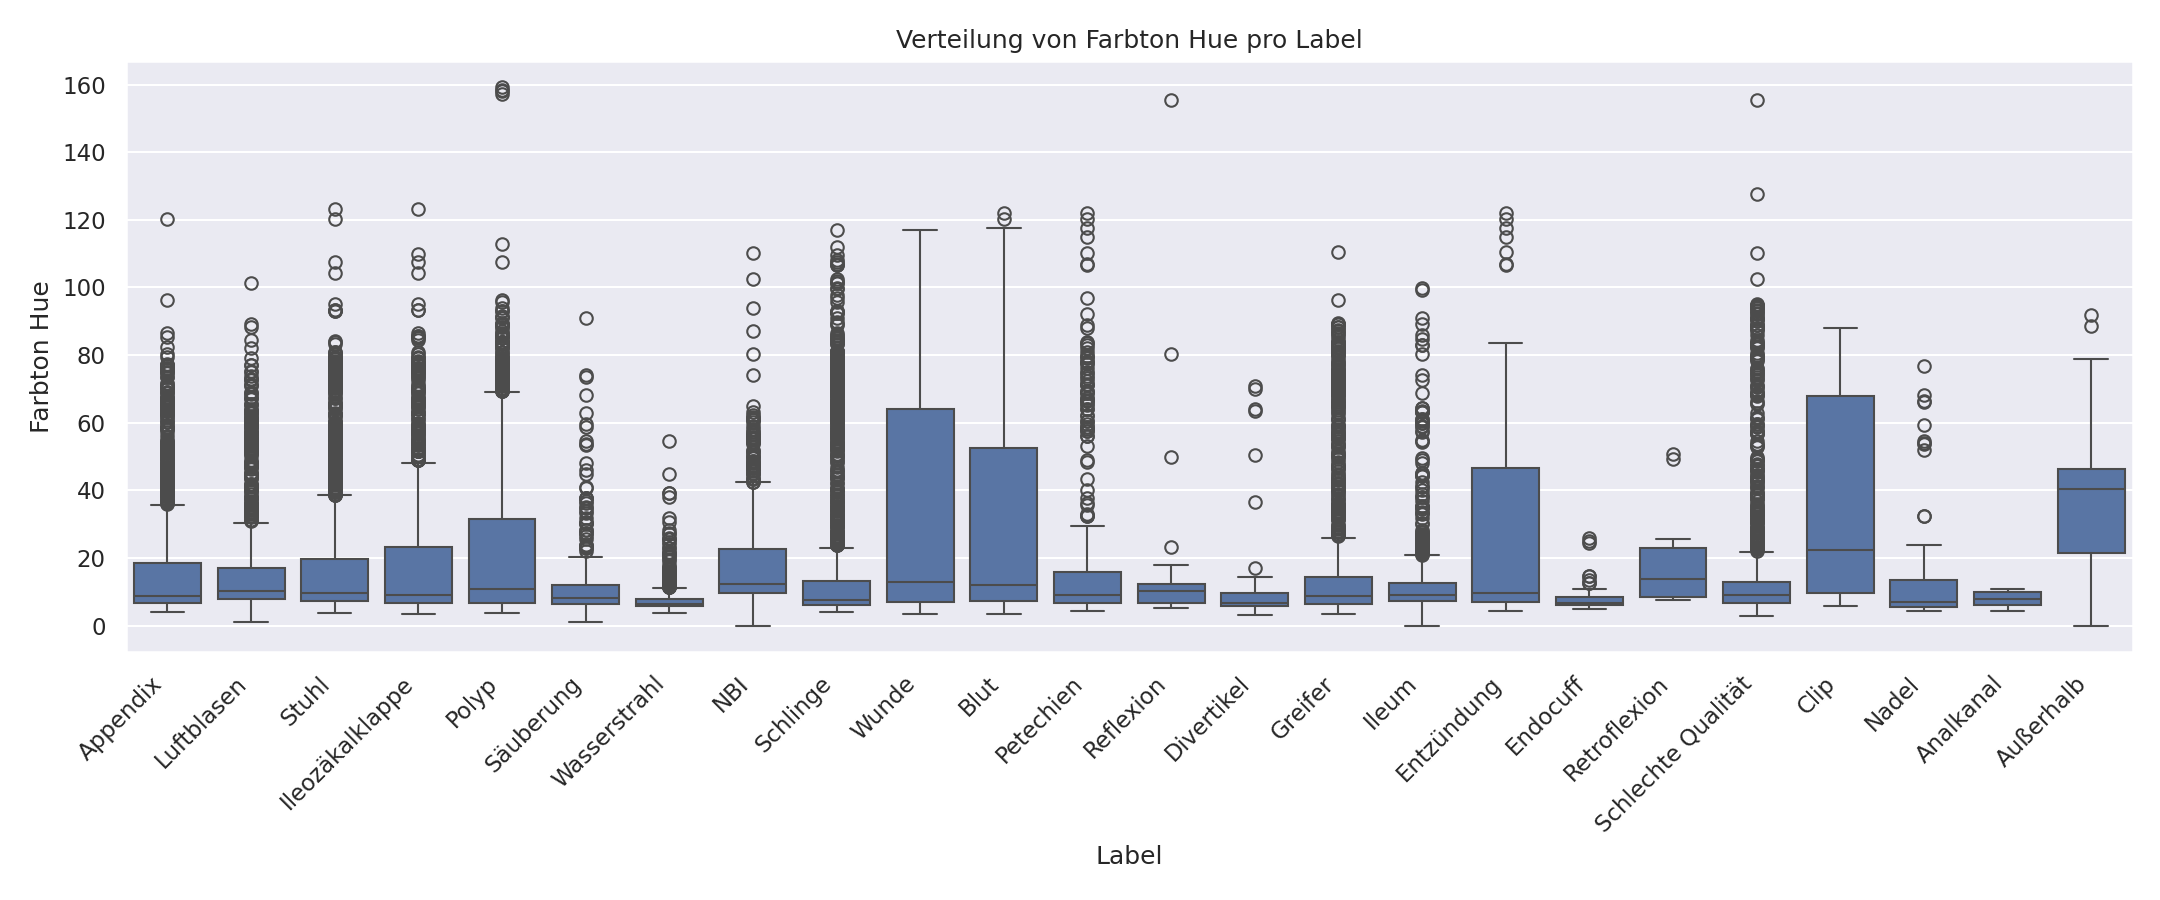
\includegraphics[width=0.9\textwidth]{Images/boxplot_hue.png}
    \caption{Boxplot der Hue-Verteilung.}
\end{figure}

\begin{figure}[p]
    \centering
    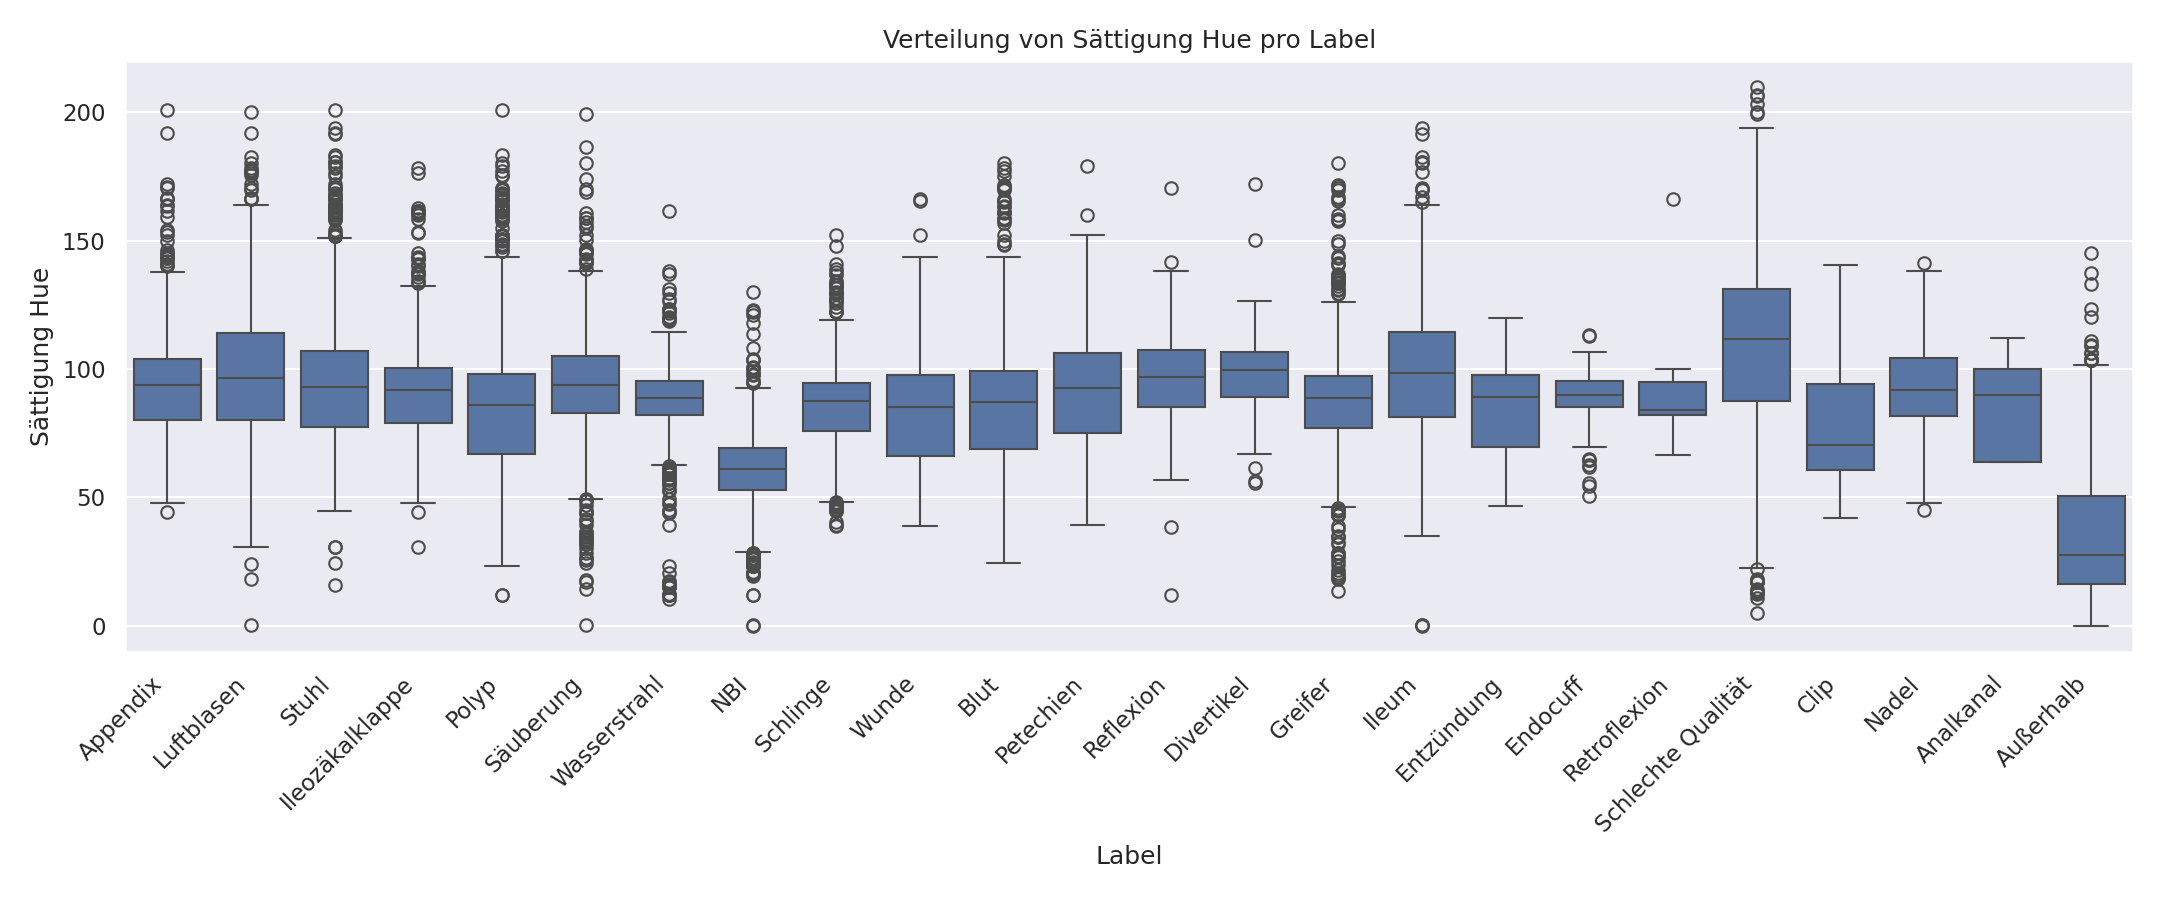
\includegraphics[width=0.9\textwidth]{Images/boxplot_saturation.png}
    \caption{Boxplot der Sättigungs-Verteilung.}
\end{figure}

\begin{figure}[p]
    \centering
    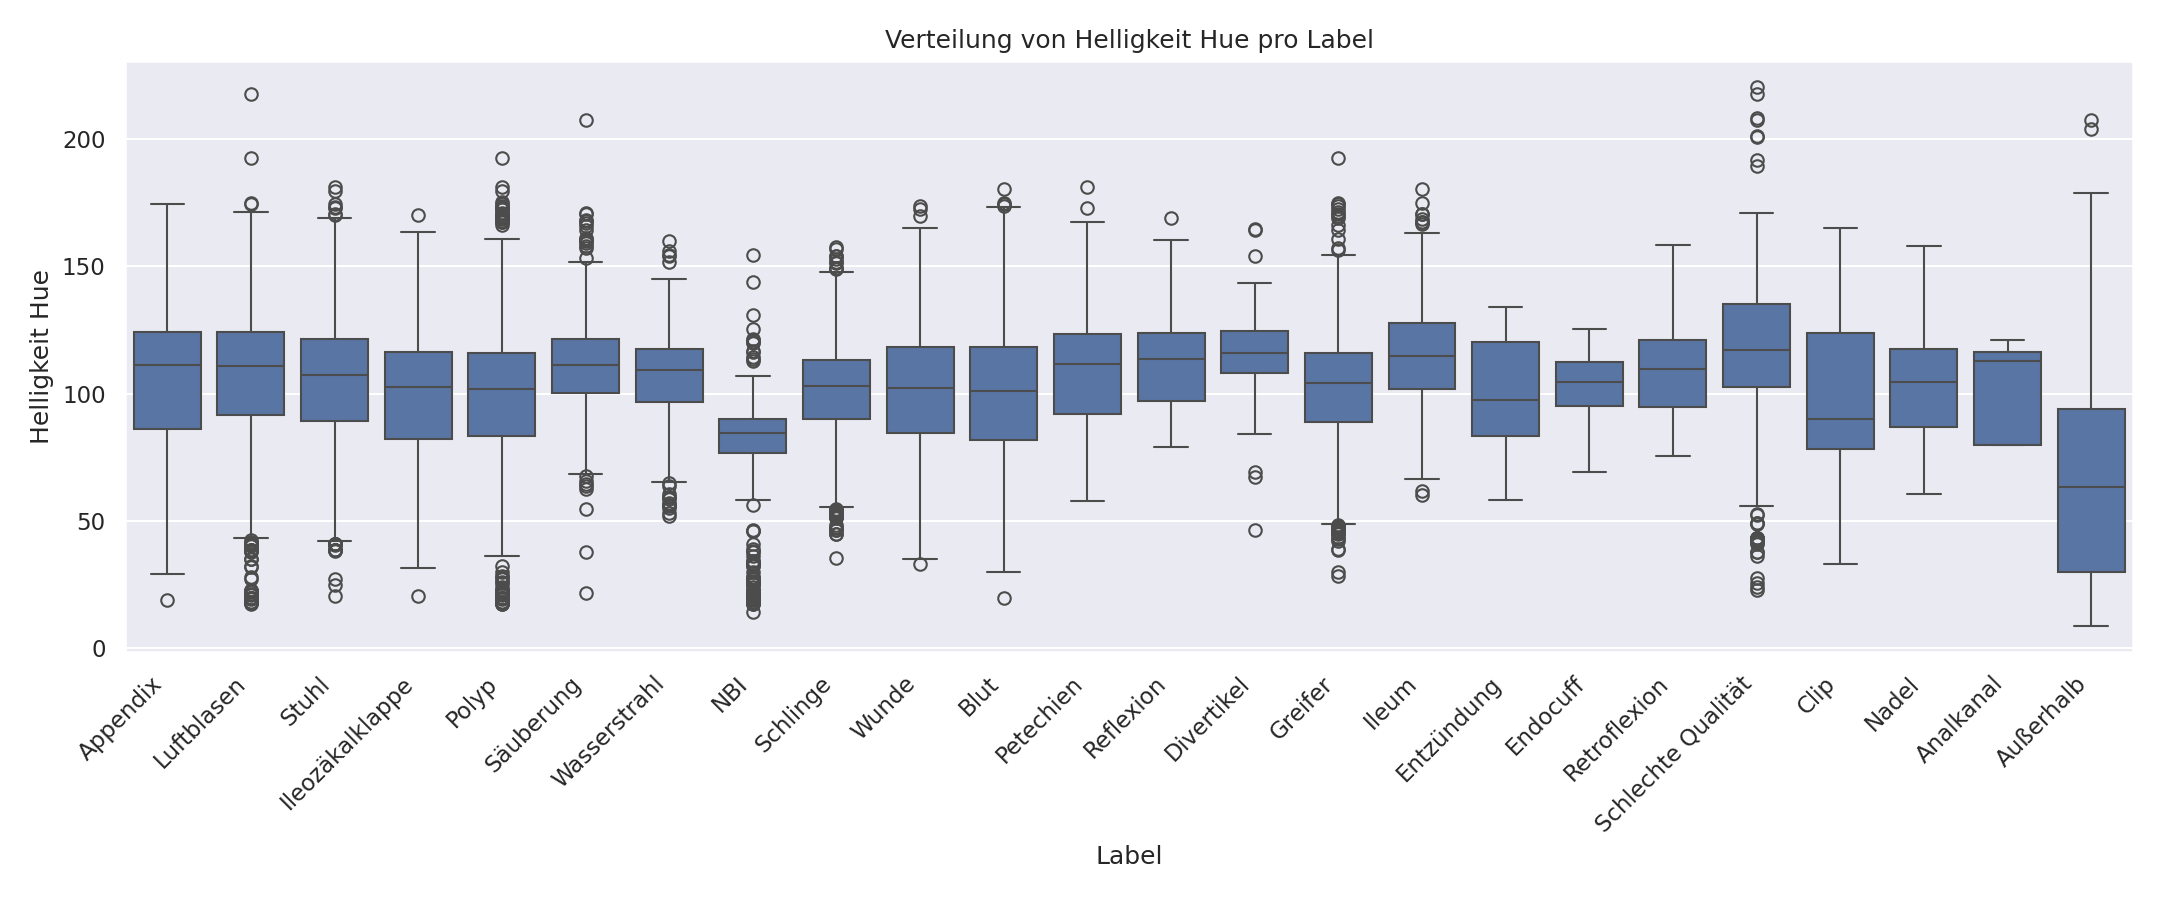
\includegraphics[width=0.9\textwidth]{Images/boxplot_value.png}
    \caption{Boxplot der Value-Verteilung.}
\end{figure}

\begin{figure}[p]
    \centering
    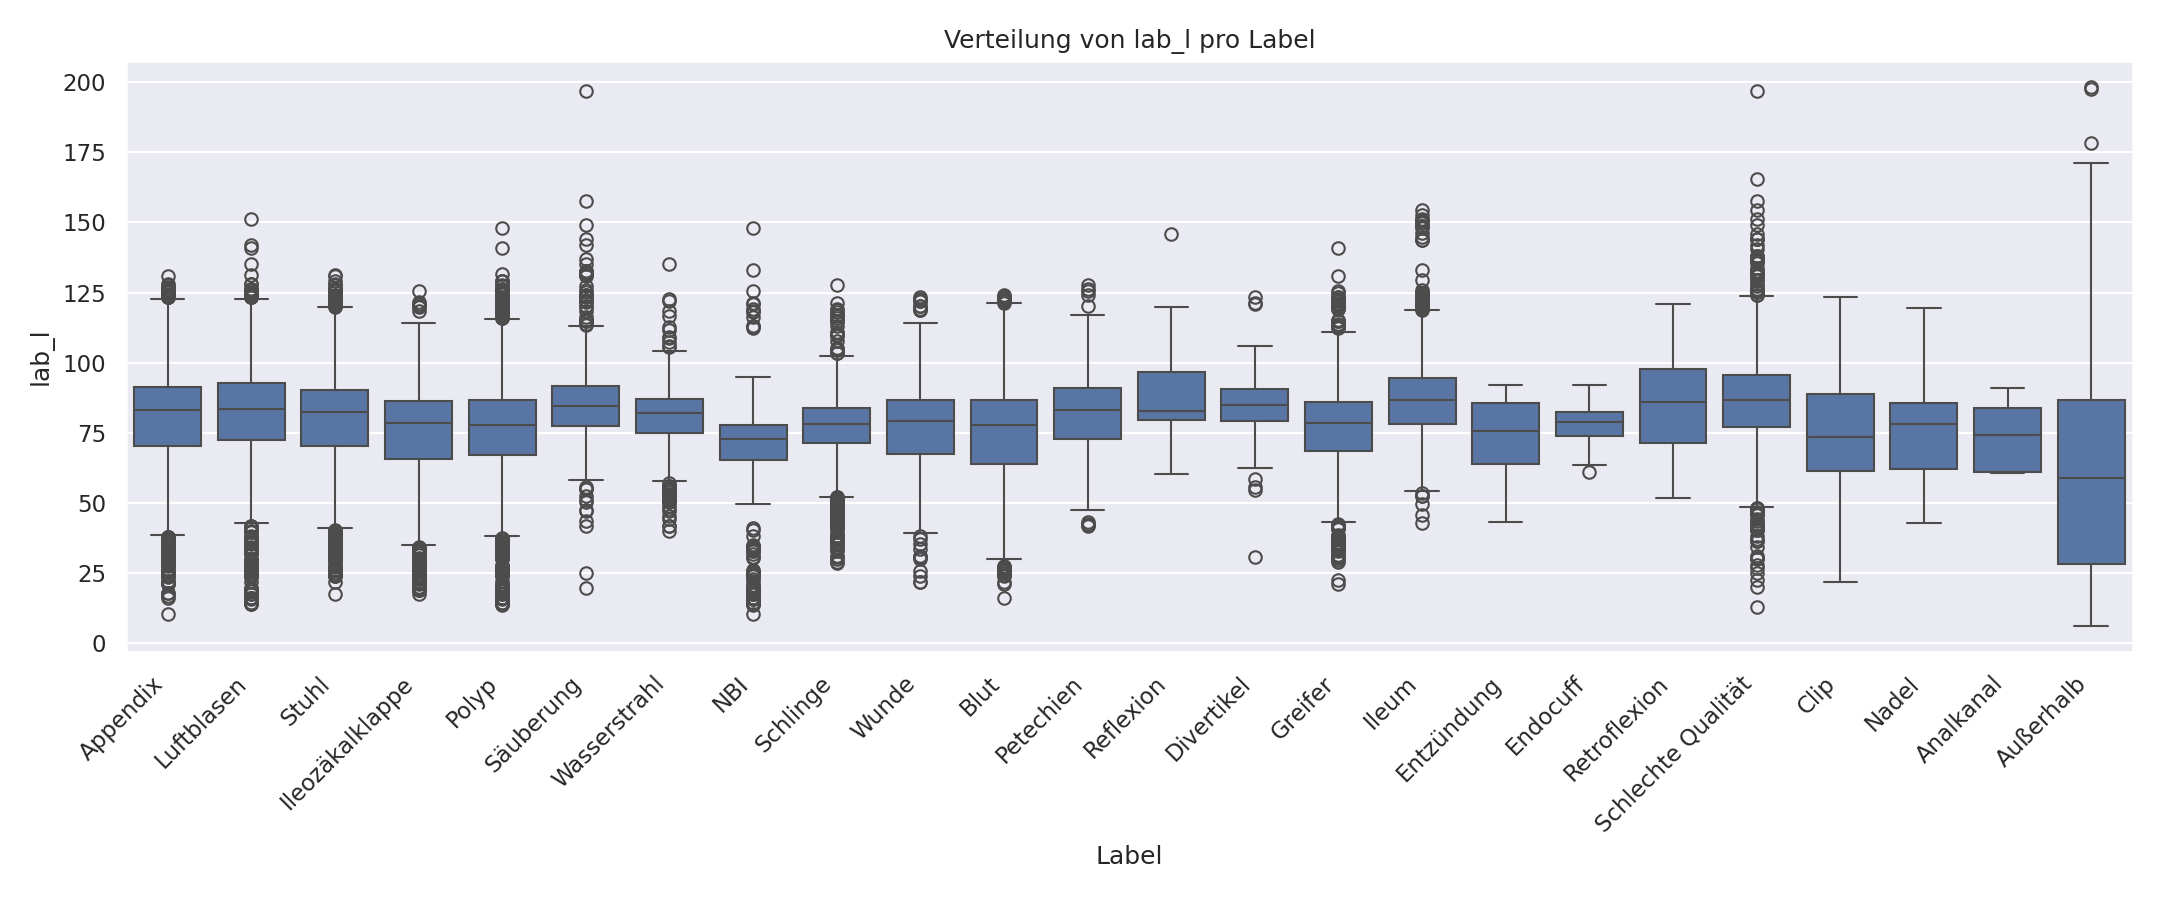
\includegraphics[width=0.9\textwidth]{Images/boxplot_lab_l.png}
    \caption{Boxplot der LAB-L-Verteilung.}
\end{figure}

\begin{figure}[p]
    \centering
    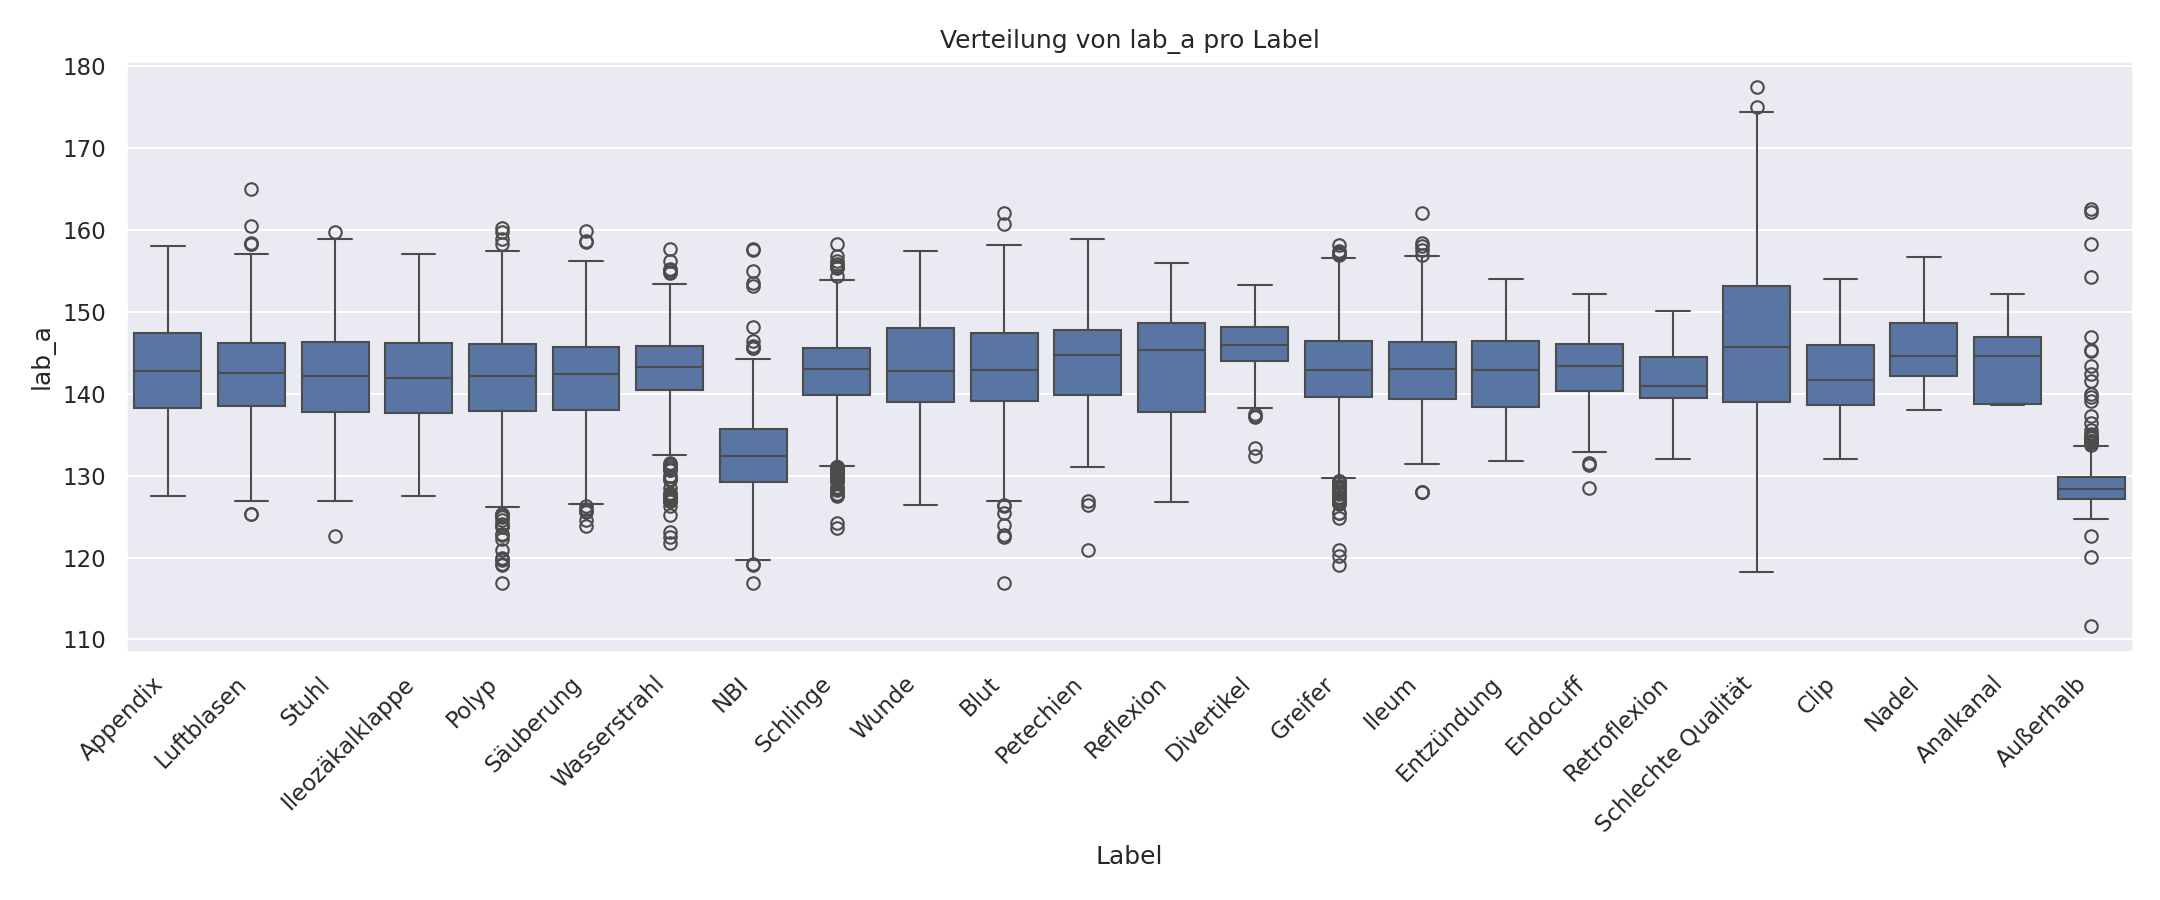
\includegraphics[width=0.9\textwidth]{Images/boxplot_lab_a.png}
    \caption{Boxplot der LAB-a-Verteilung.}
\end{figure}

\begin{figure}[p]
    \centering
    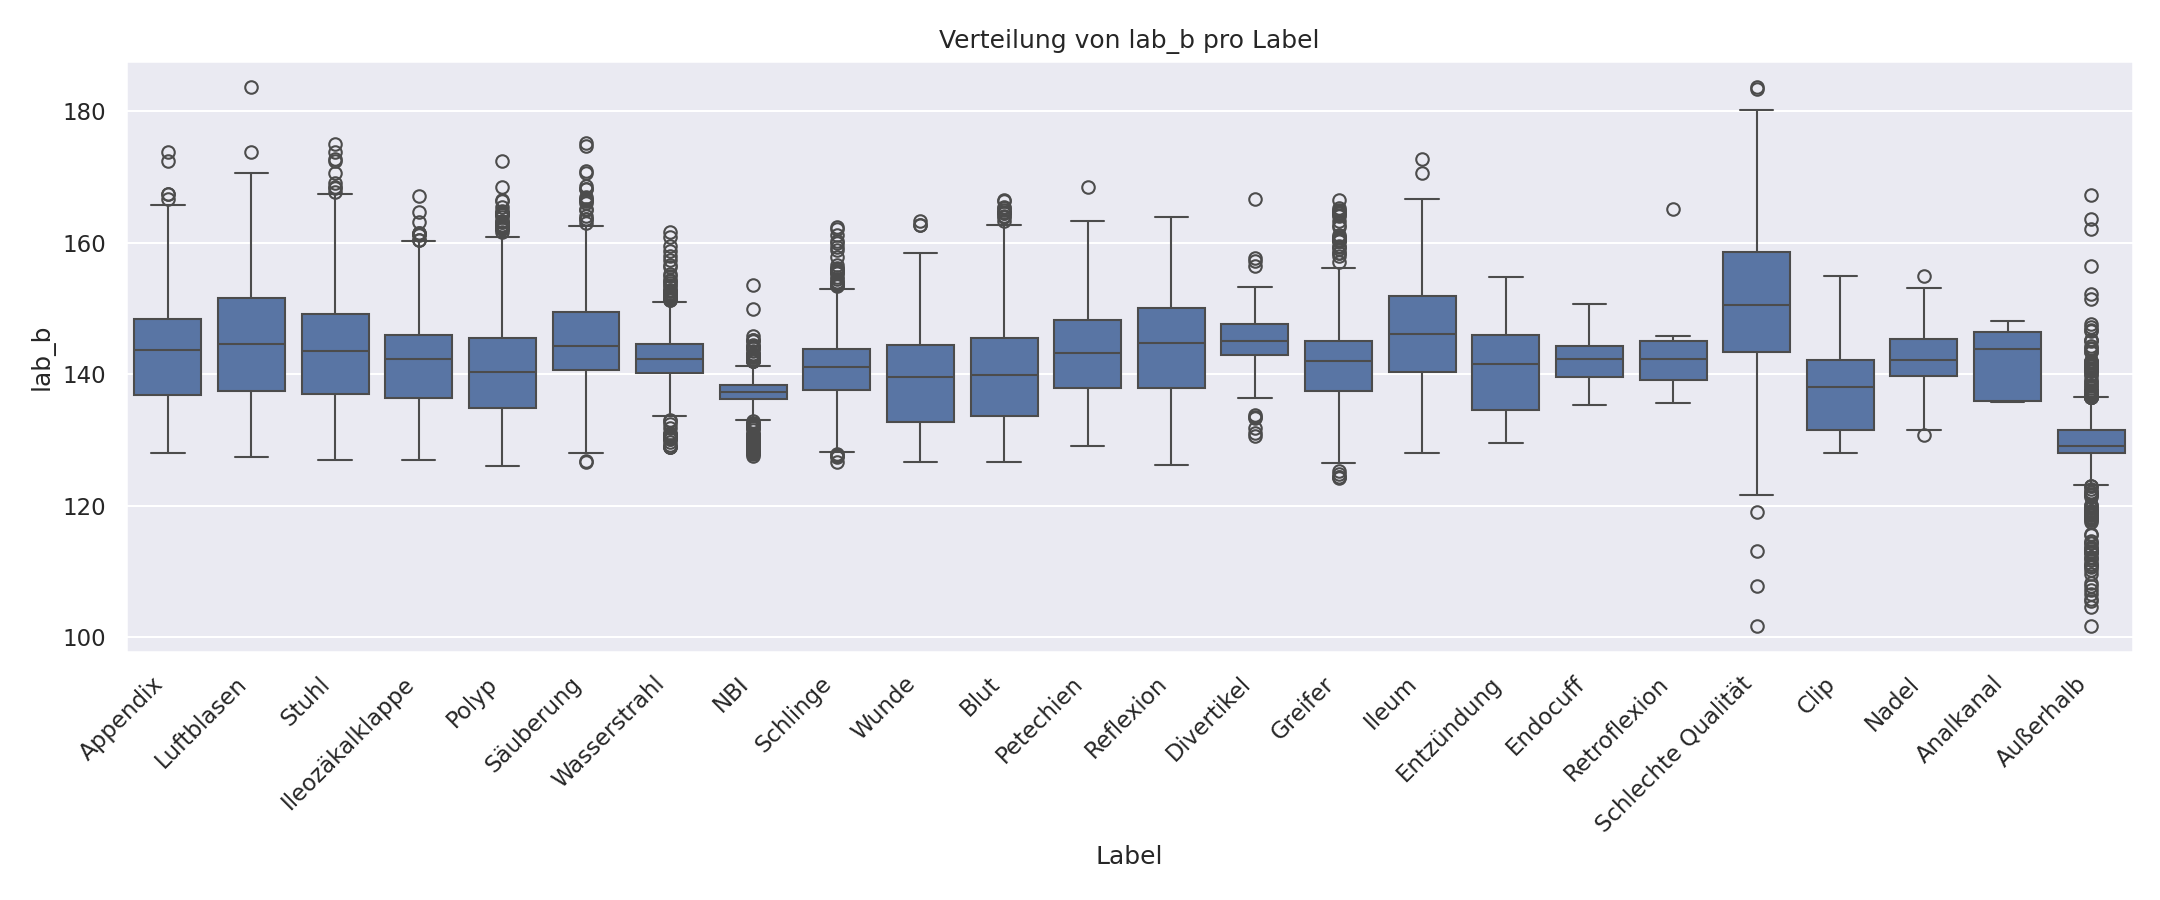
\includegraphics[width=0.9\textwidth]{Images/boxplot_lab_b.png}
    \caption{Boxplot der LAB-b-Verteilung.}
\end{figure}

\begin{figure}[p]
    \centering
    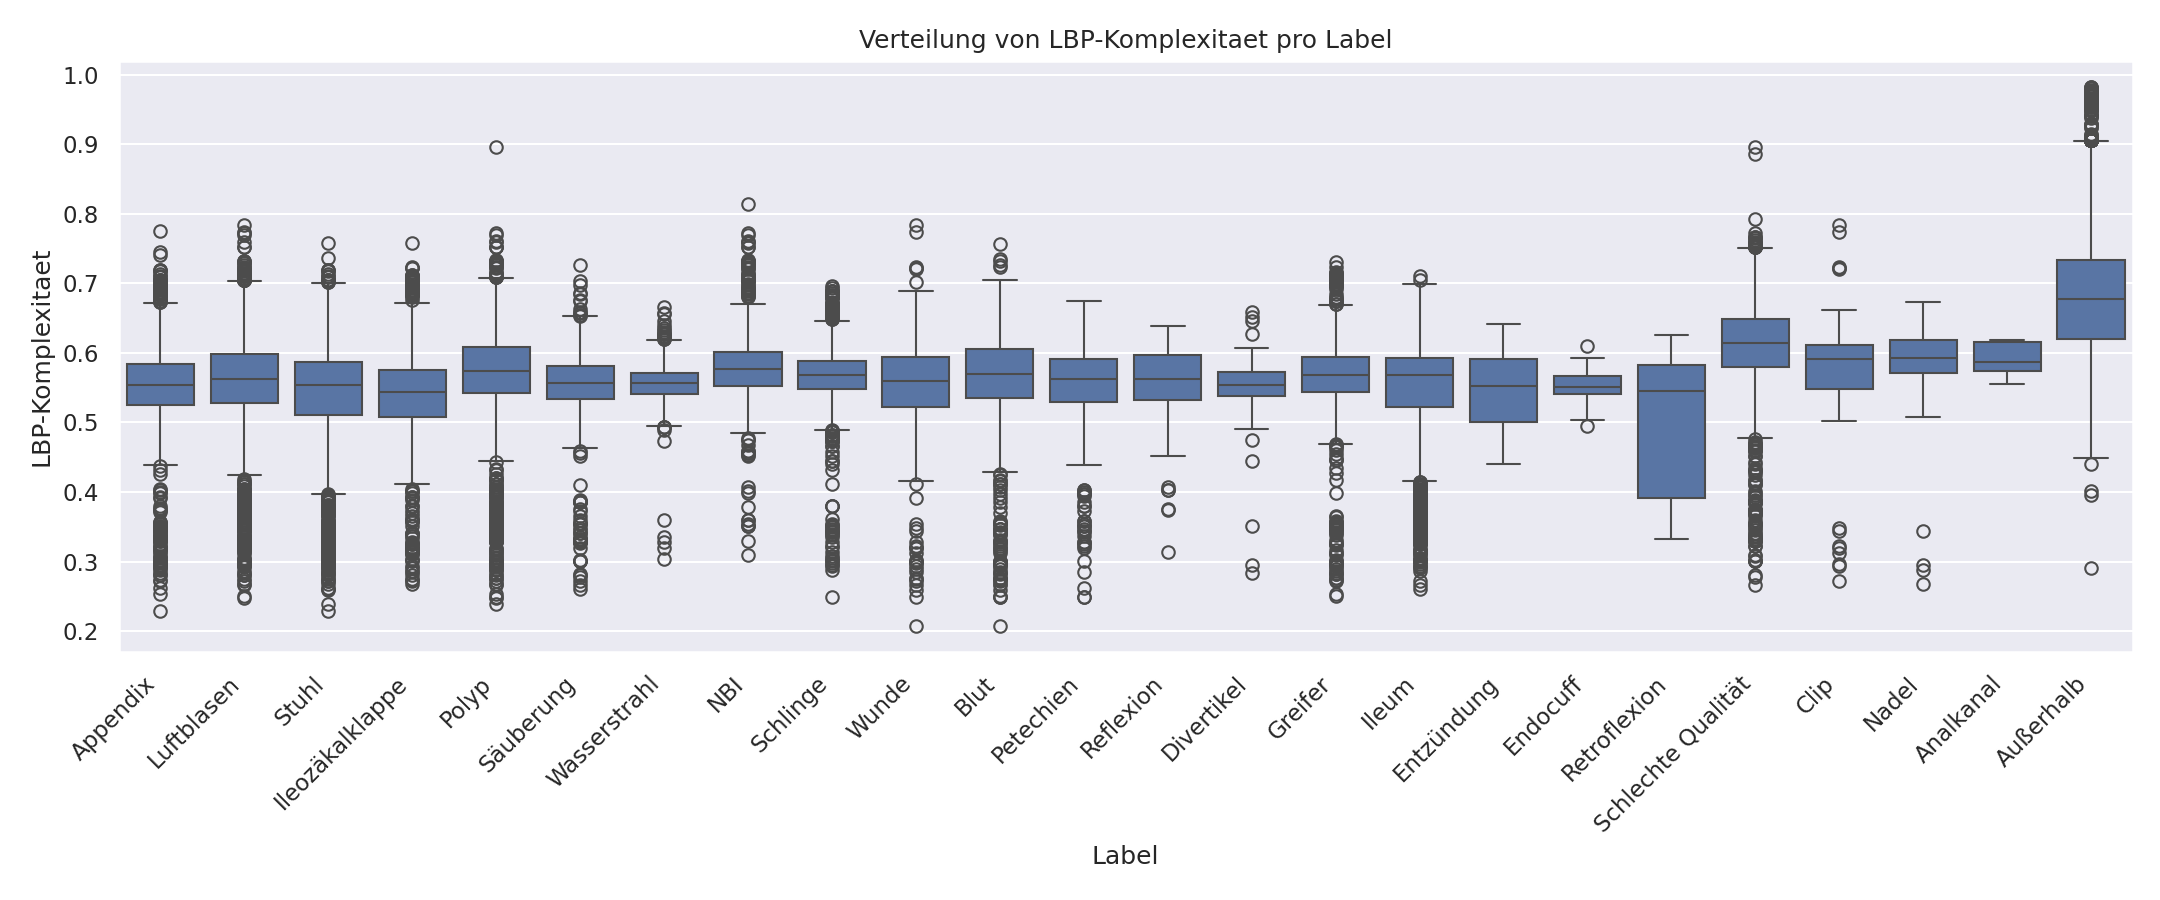
\includegraphics[width=0.9\textwidth]{Images/boxplot_texture_lbp_complexity.png}
    \caption{Boxplot der LBP-Komplexität.}
\end{figure}

\begin{figure}[p]
    \centering
    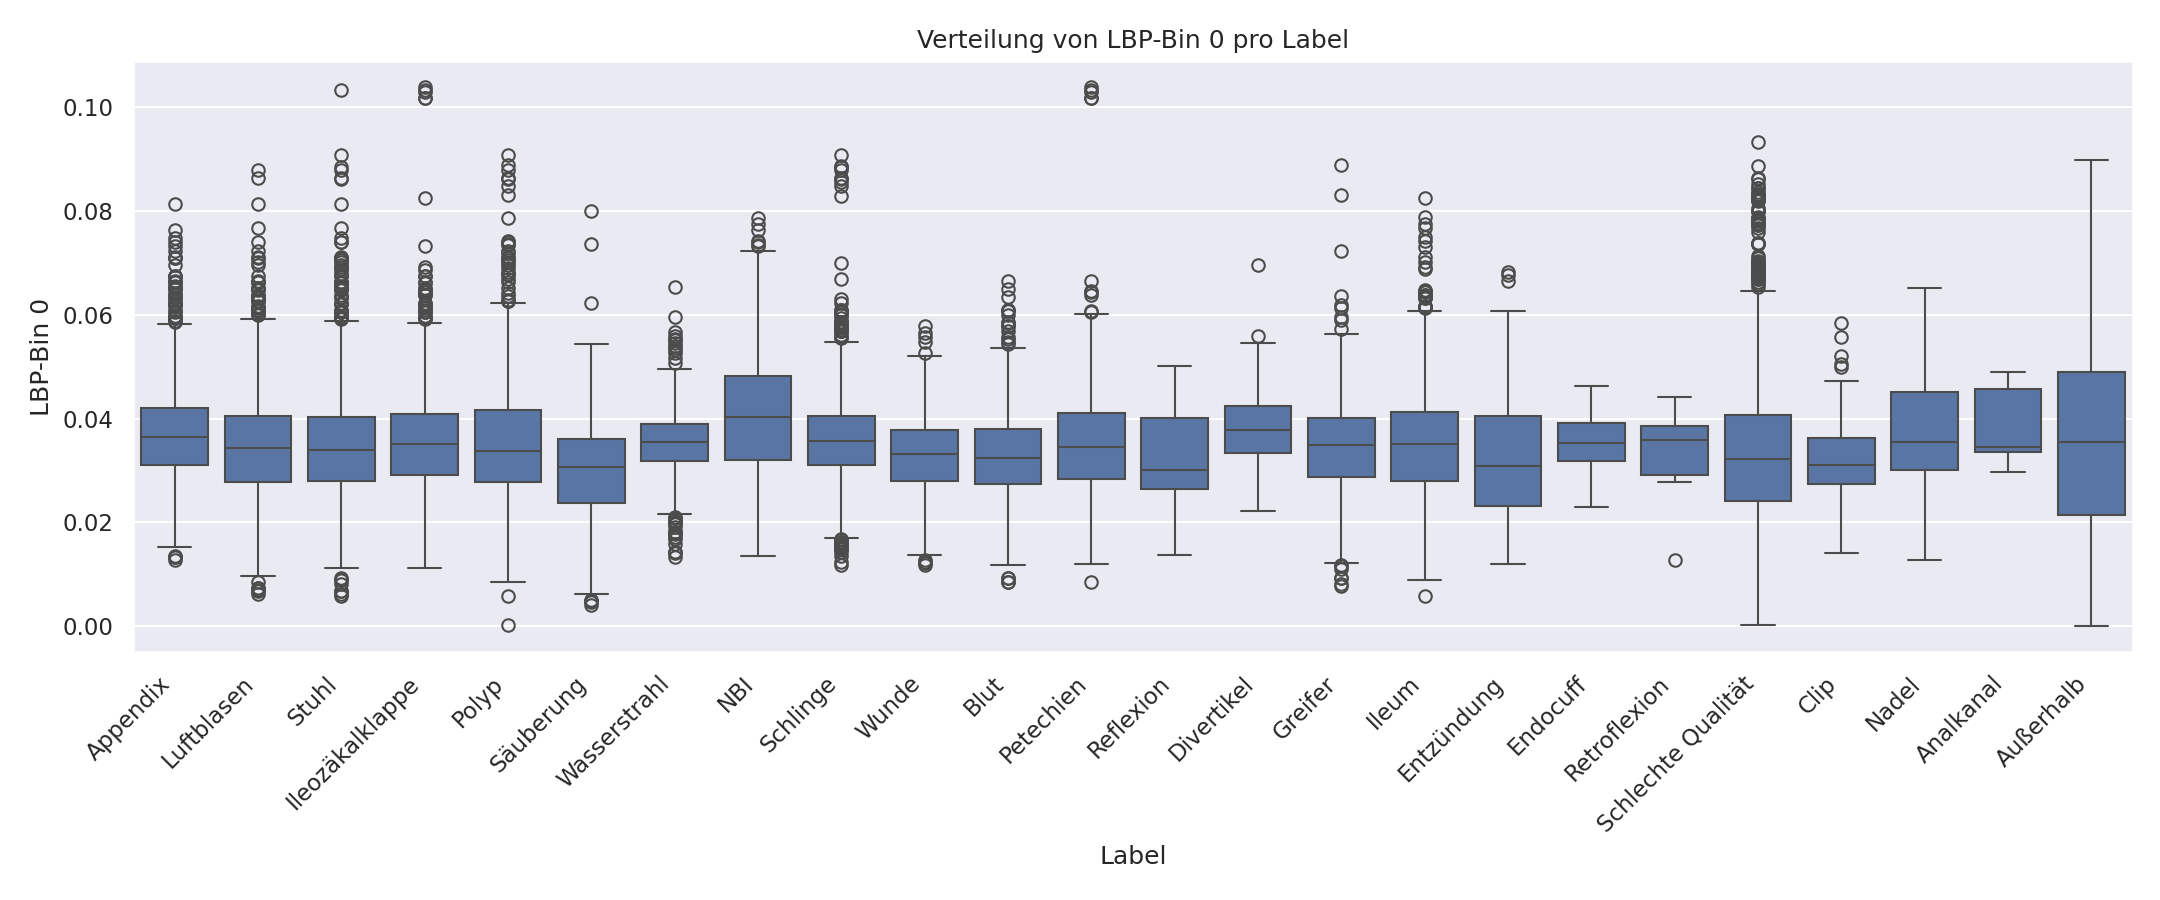
\includegraphics[width=0.9\textwidth]{Images/boxplot_texture_lbp_bin_0.png}
    \caption{Boxplot des LBP-Bins 0.}
\end{figure}

\begin{figure}[p]
    \centering
    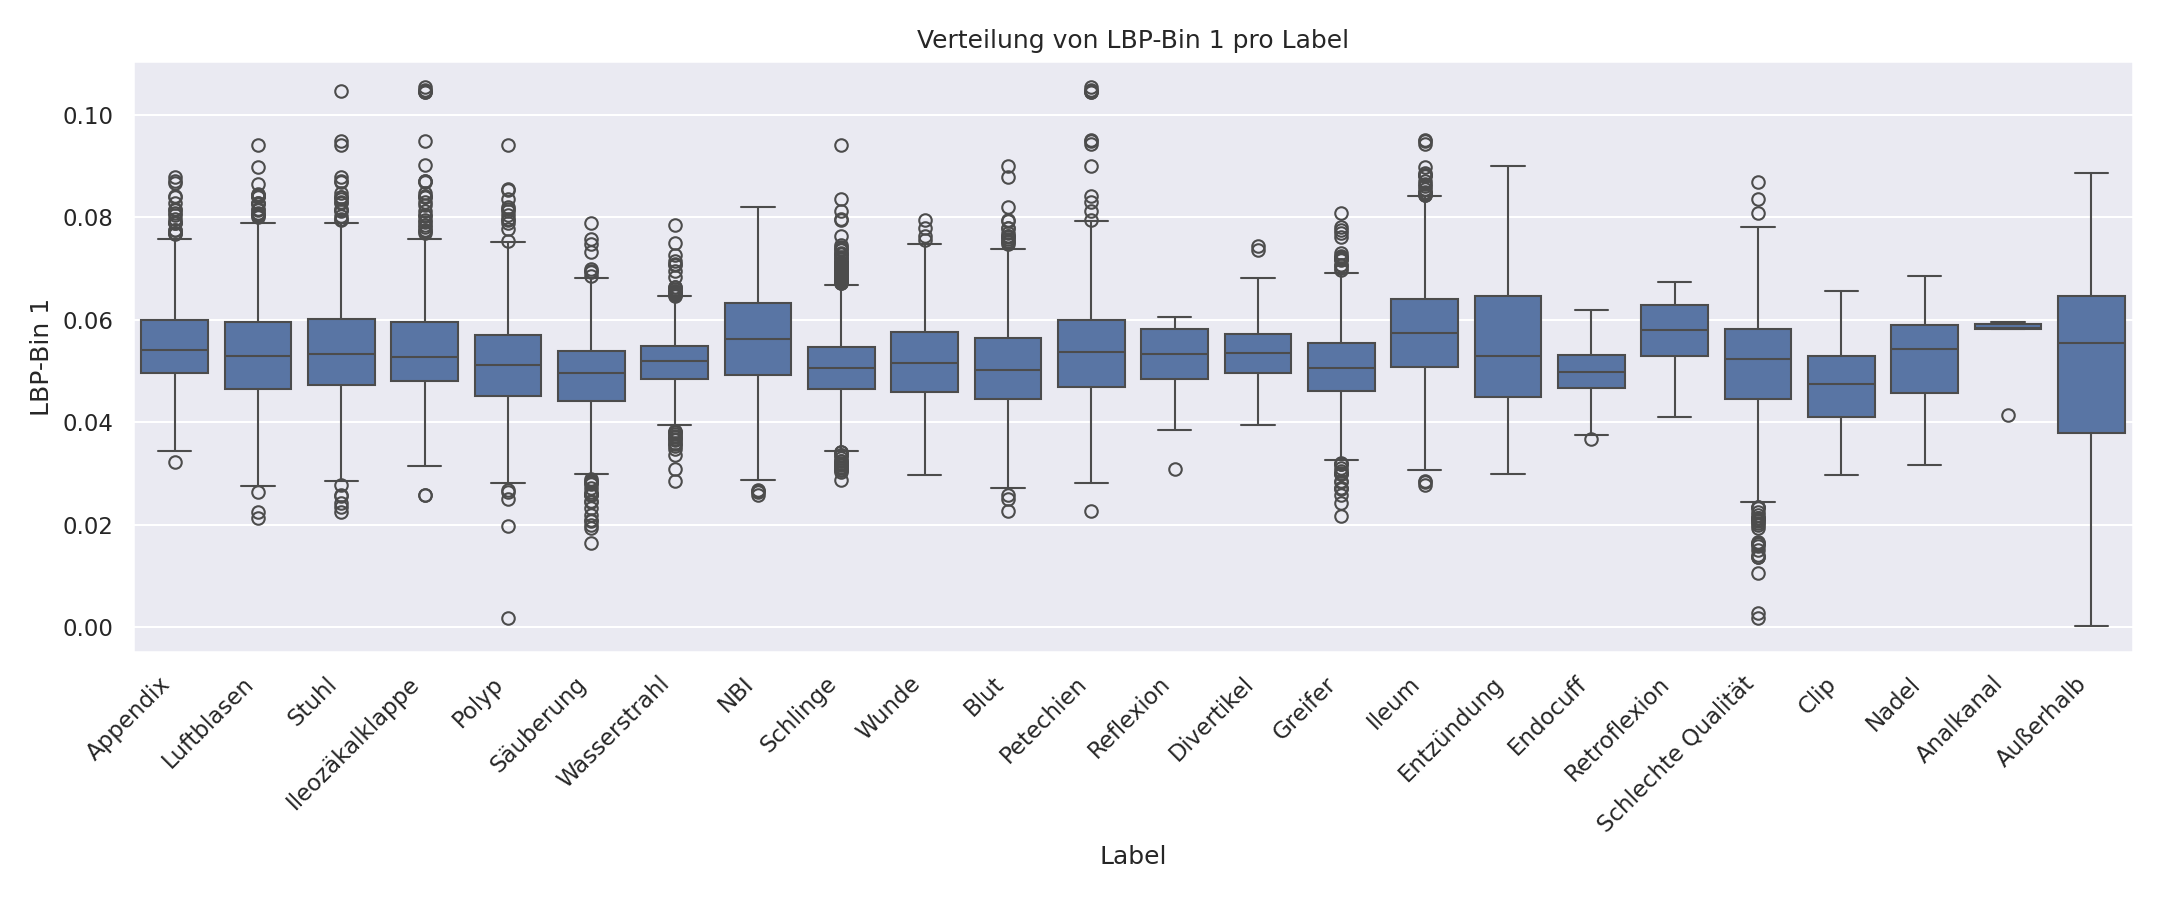
\includegraphics[width=0.9\textwidth]{Images/boxplot_texture_lbp_bin_1.png}
    \caption{Boxplot des LBP-Bins 1.}
\end{figure}

\begin{figure}[p]
    \centering
    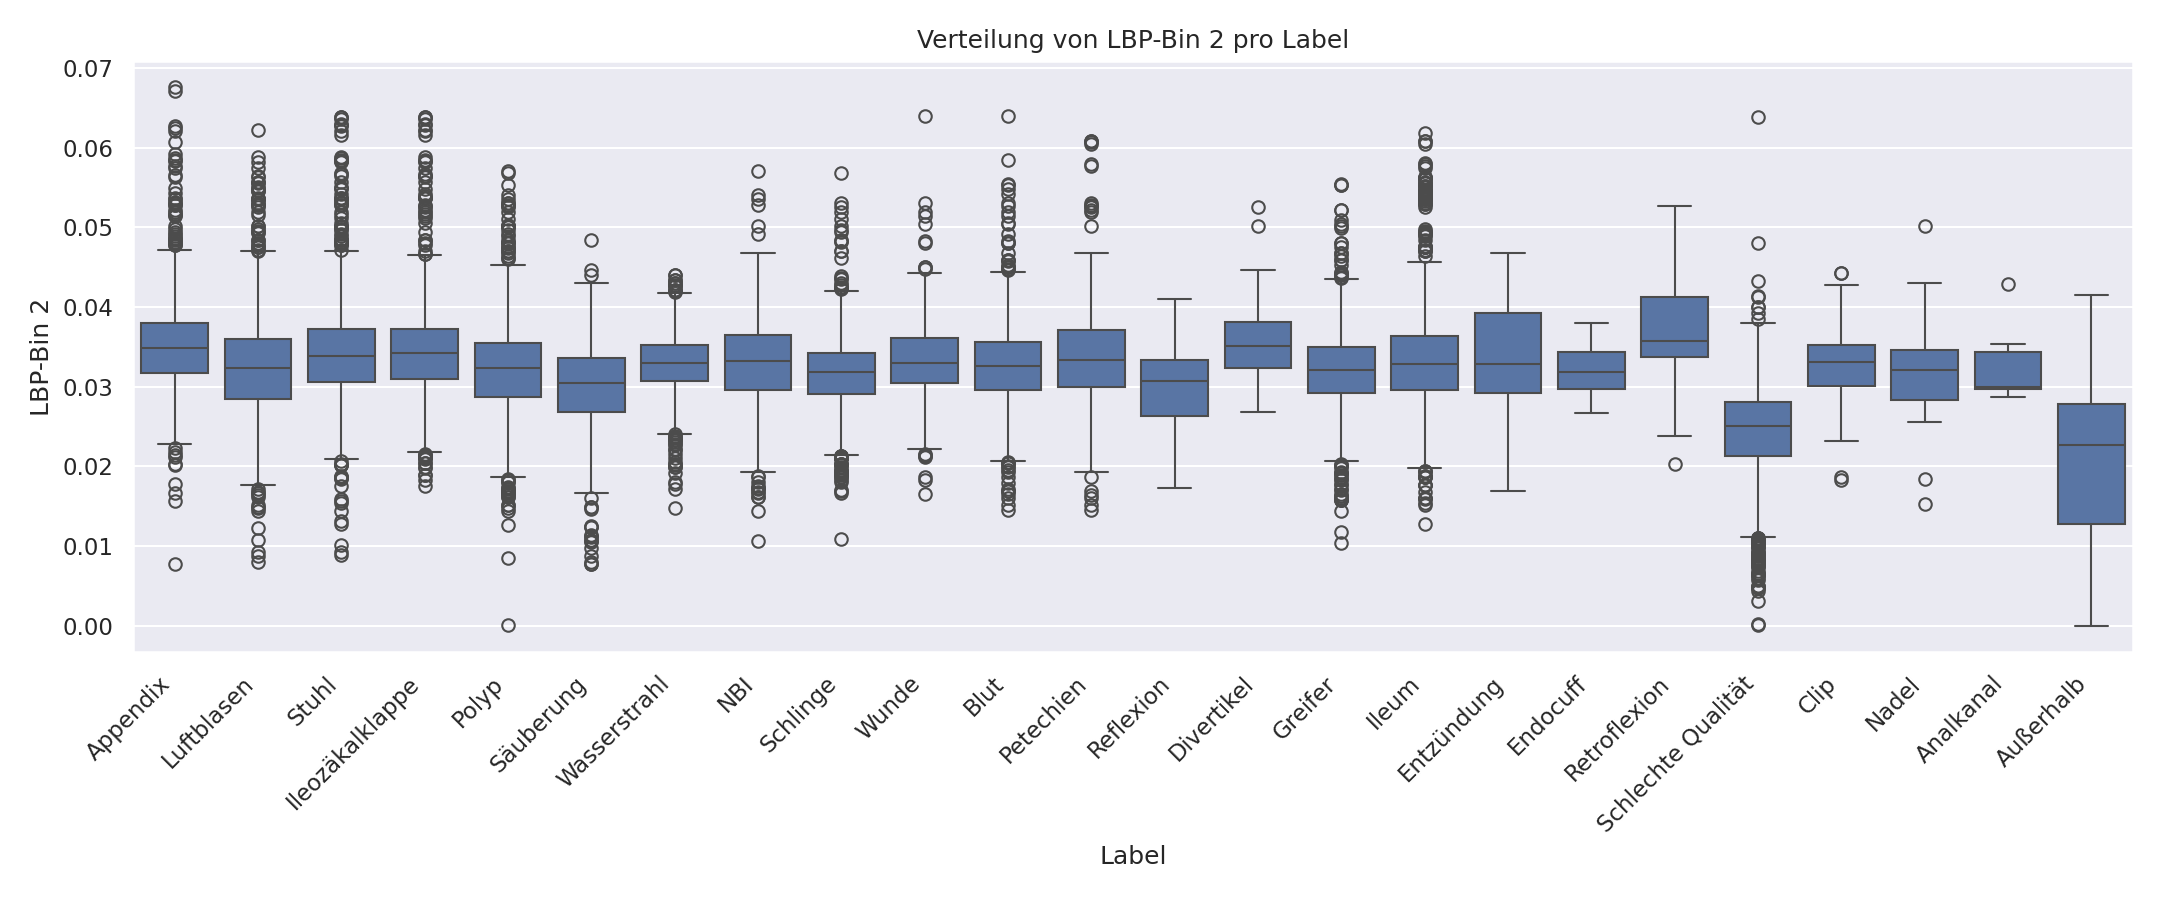
\includegraphics[width=0.9\textwidth]{Images/boxplot_texture_lbp_bin_2.png}
    \caption{Boxplot des LBP-Bins 2.}
\end{figure}

\begin{figure}[p]
    \centering
    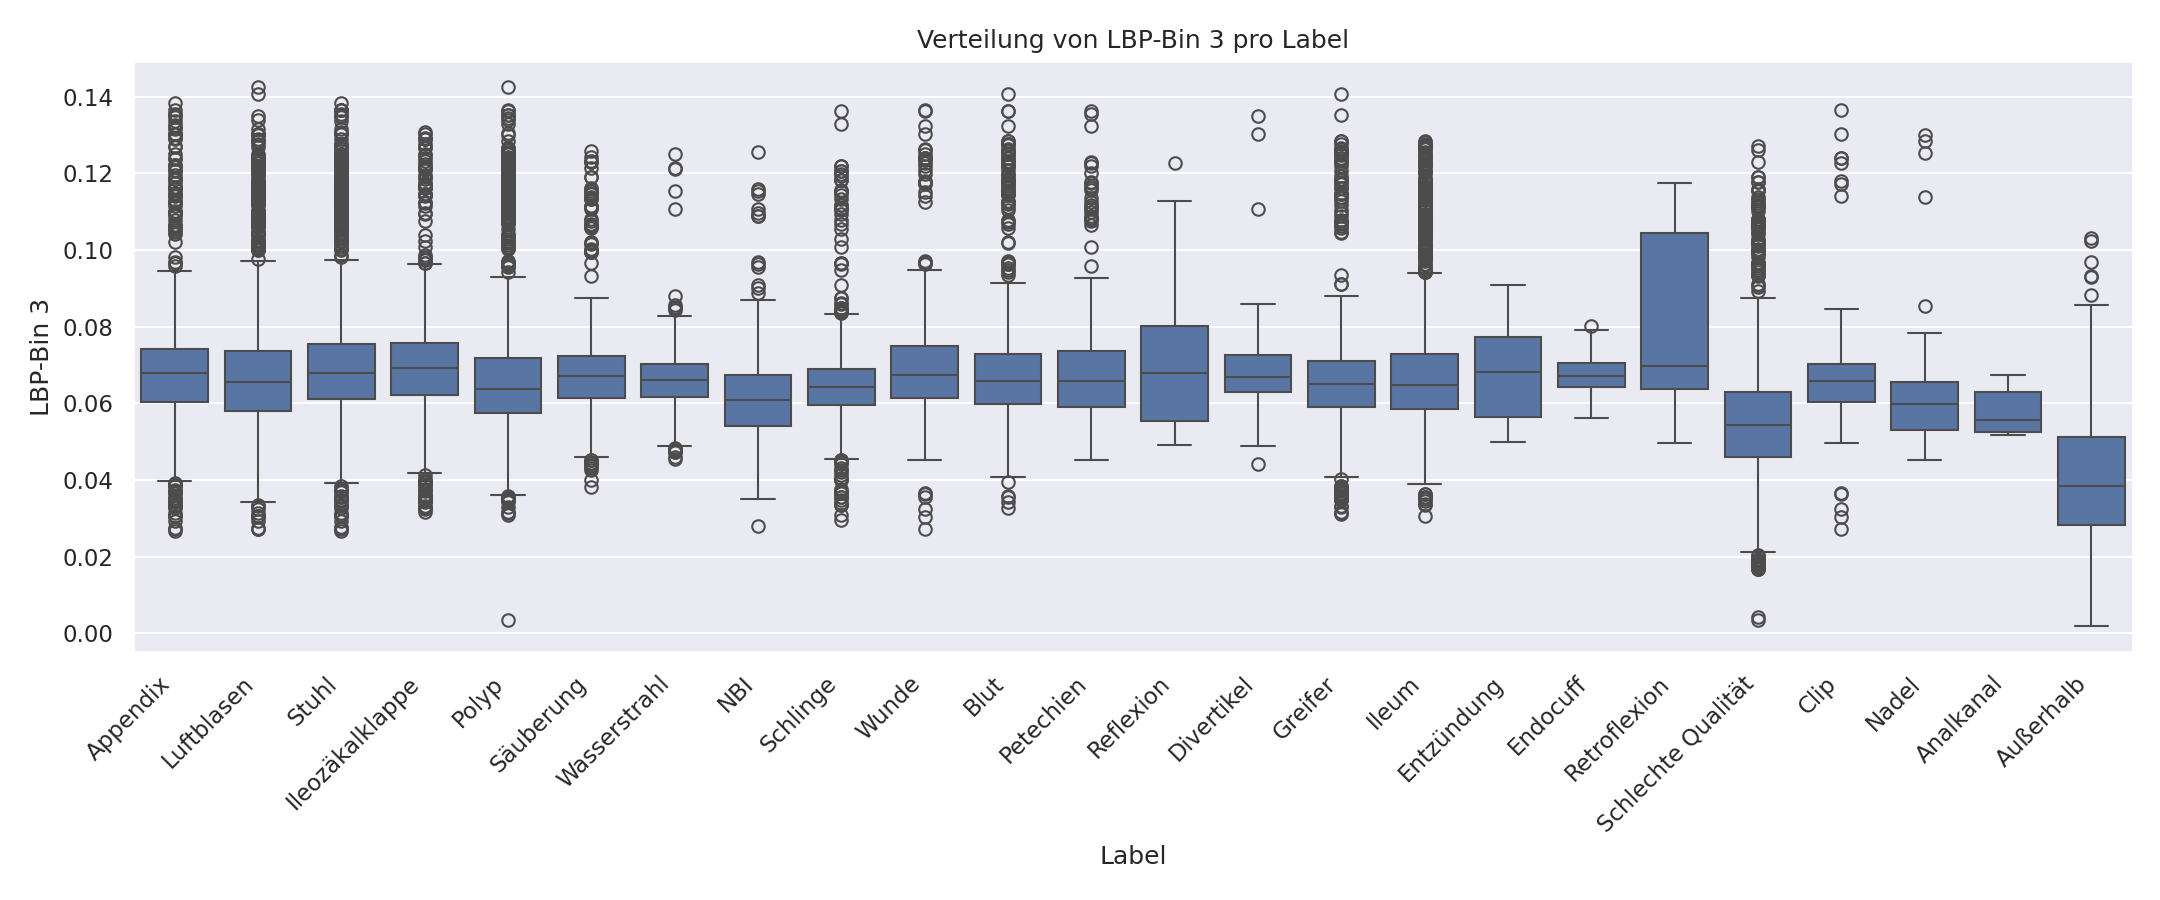
\includegraphics[width=0.9\textwidth]{Images/boxplot_texture_lbp_bin_3.png}
    \caption{Boxplot des LBP-Bins 3.}
\end{figure}

\begin{figure}[p]
    \centering
    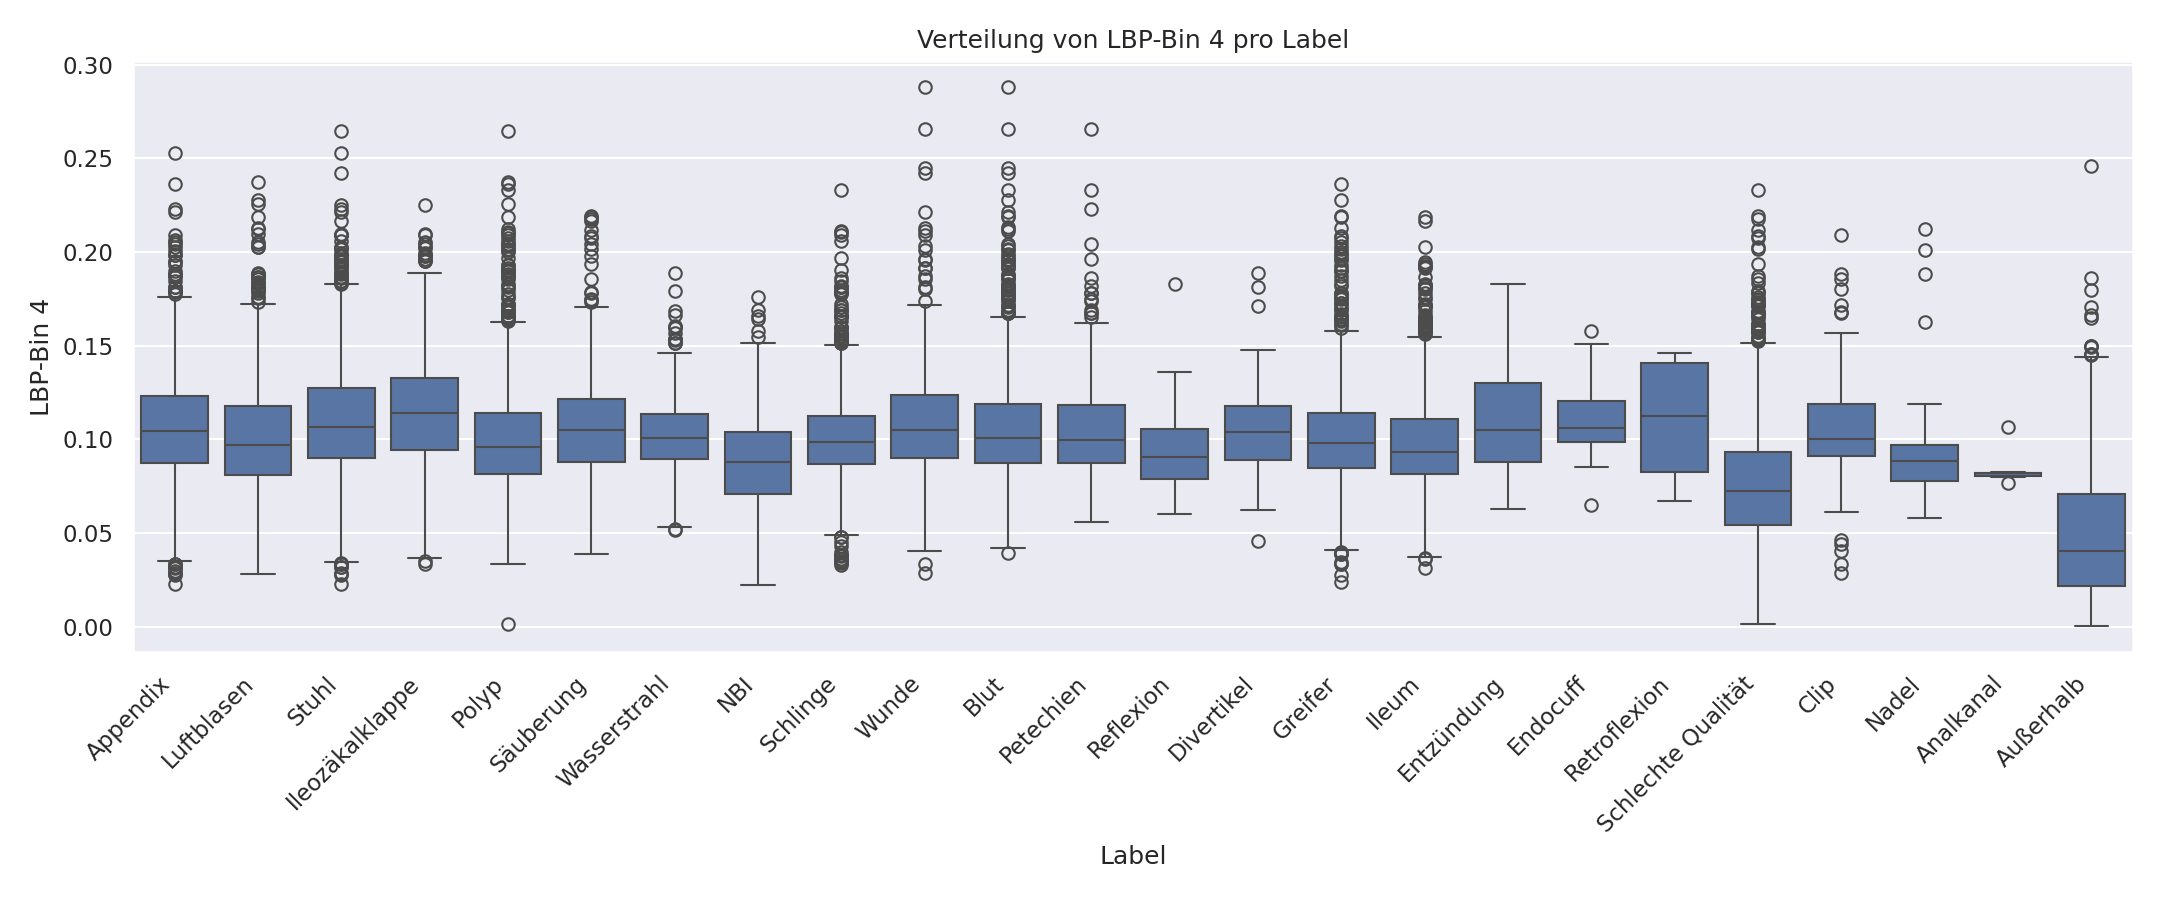
\includegraphics[width=0.9\textwidth]{Images/boxplot_texture_lbp_bin_4.png}
    \caption{Boxplot des LBP-Bins 4.}
\end{figure}

\begin{figure}[p]
    \centering
    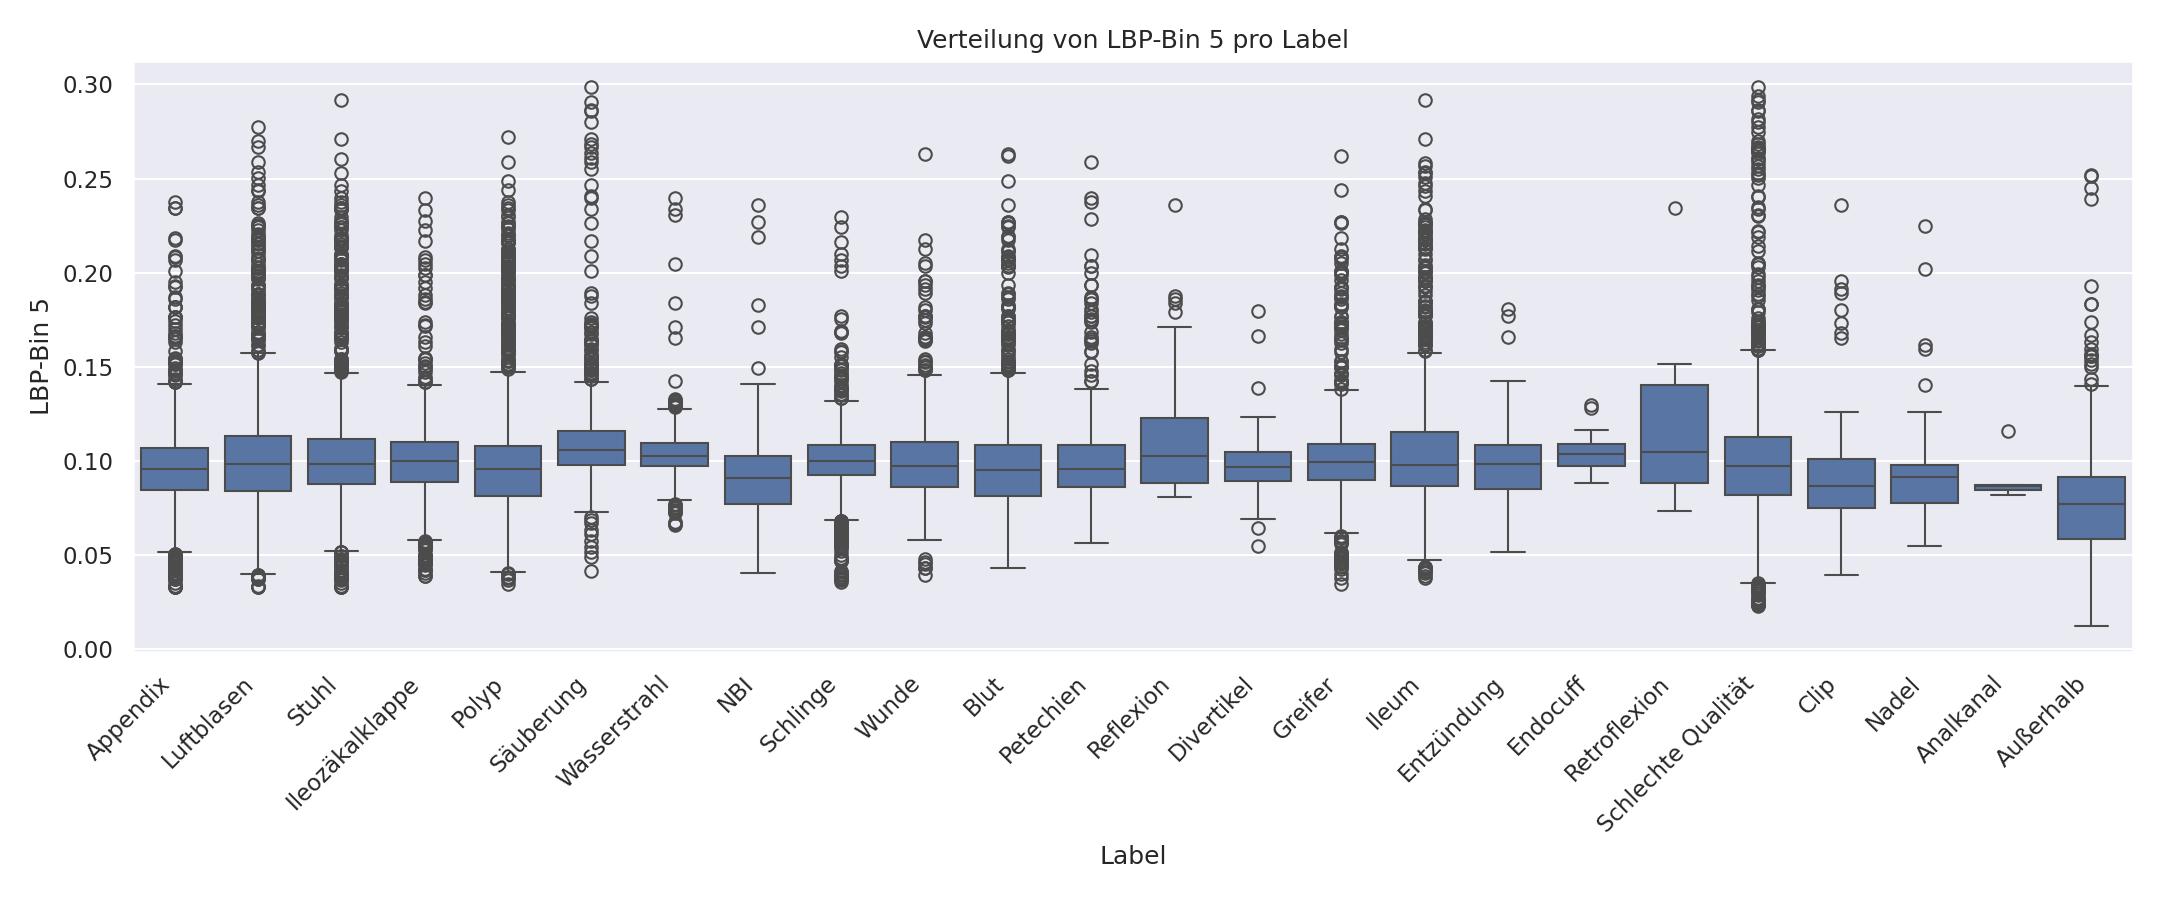
\includegraphics[width=0.9\textwidth]{Images/boxplot_texture_lbp_bin_5.png}
    \caption{Boxplot des LBP-Bins 5.}
\end{figure}

\begin{figure}[p]
    \centering
    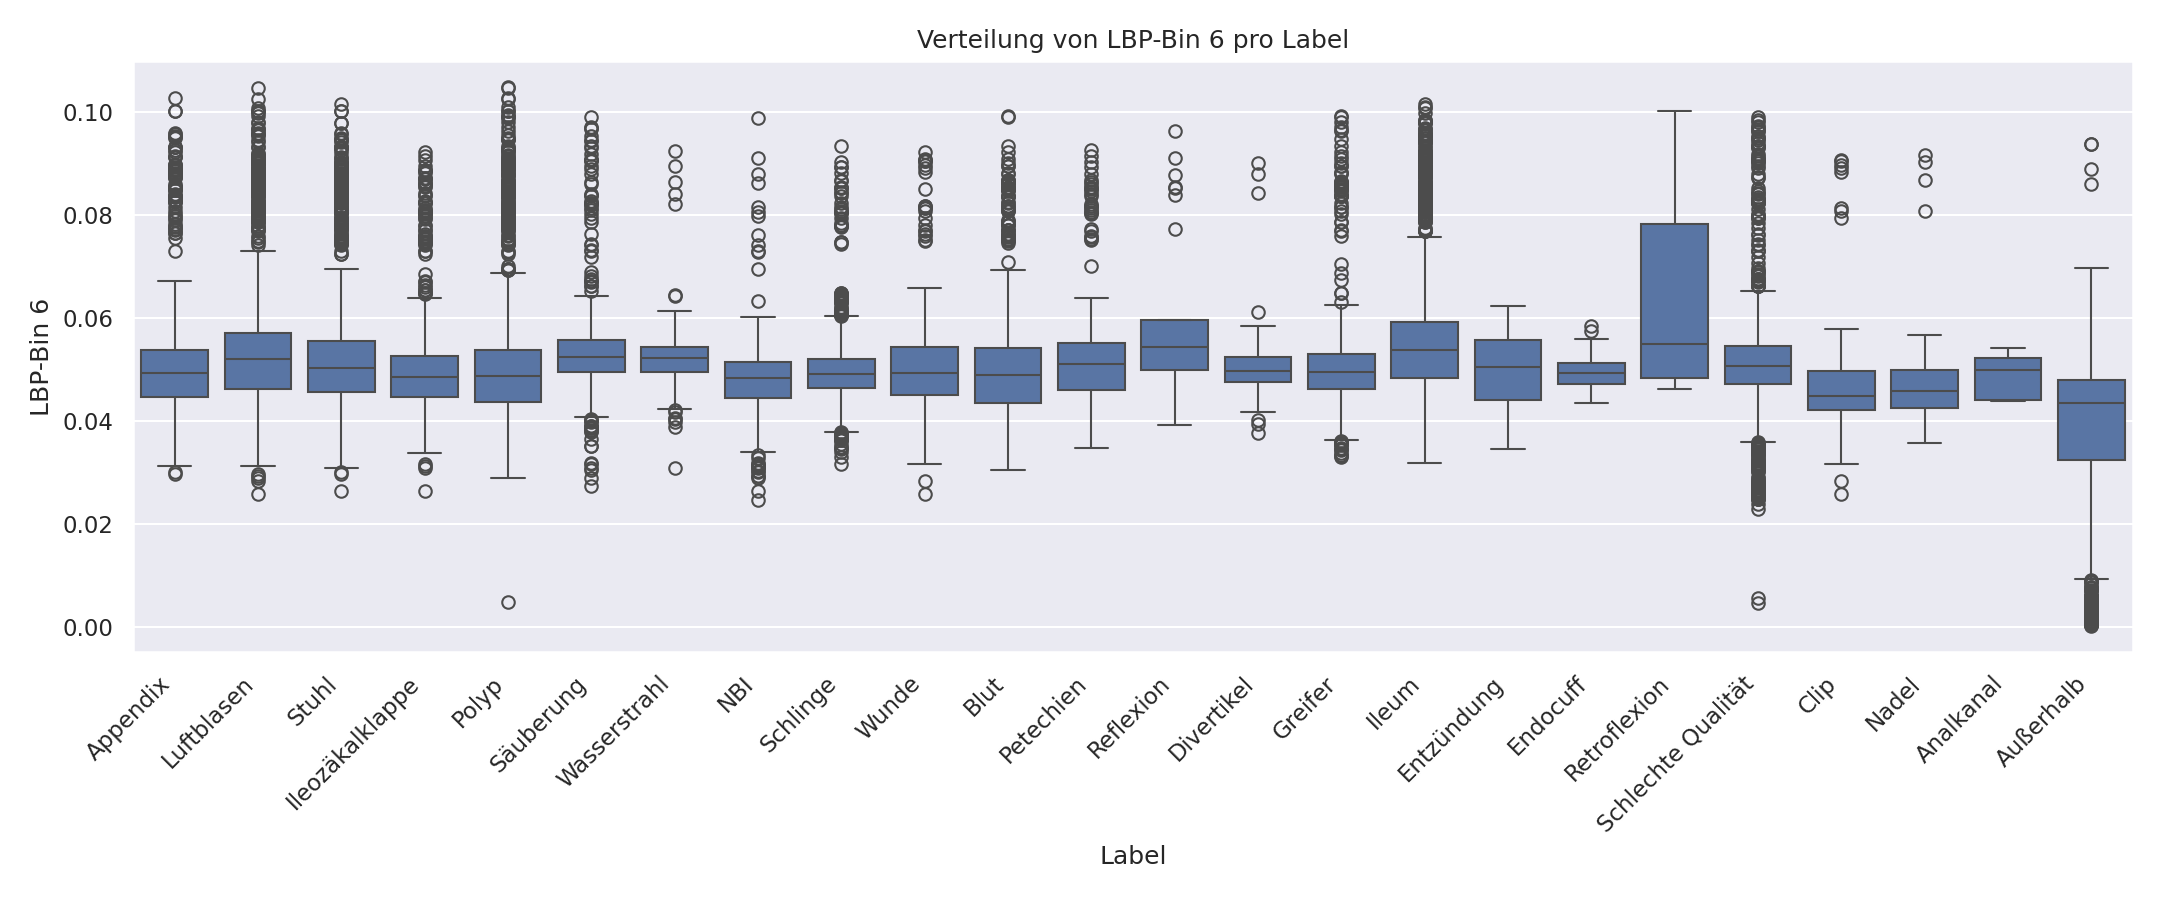
\includegraphics[width=0.9\textwidth]{Images/boxplot_texture_lbp_bin_6.png}
    \caption{Boxplot des LBP-Bins 6.}
\end{figure}

\begin{figure}[p]
    \centering
    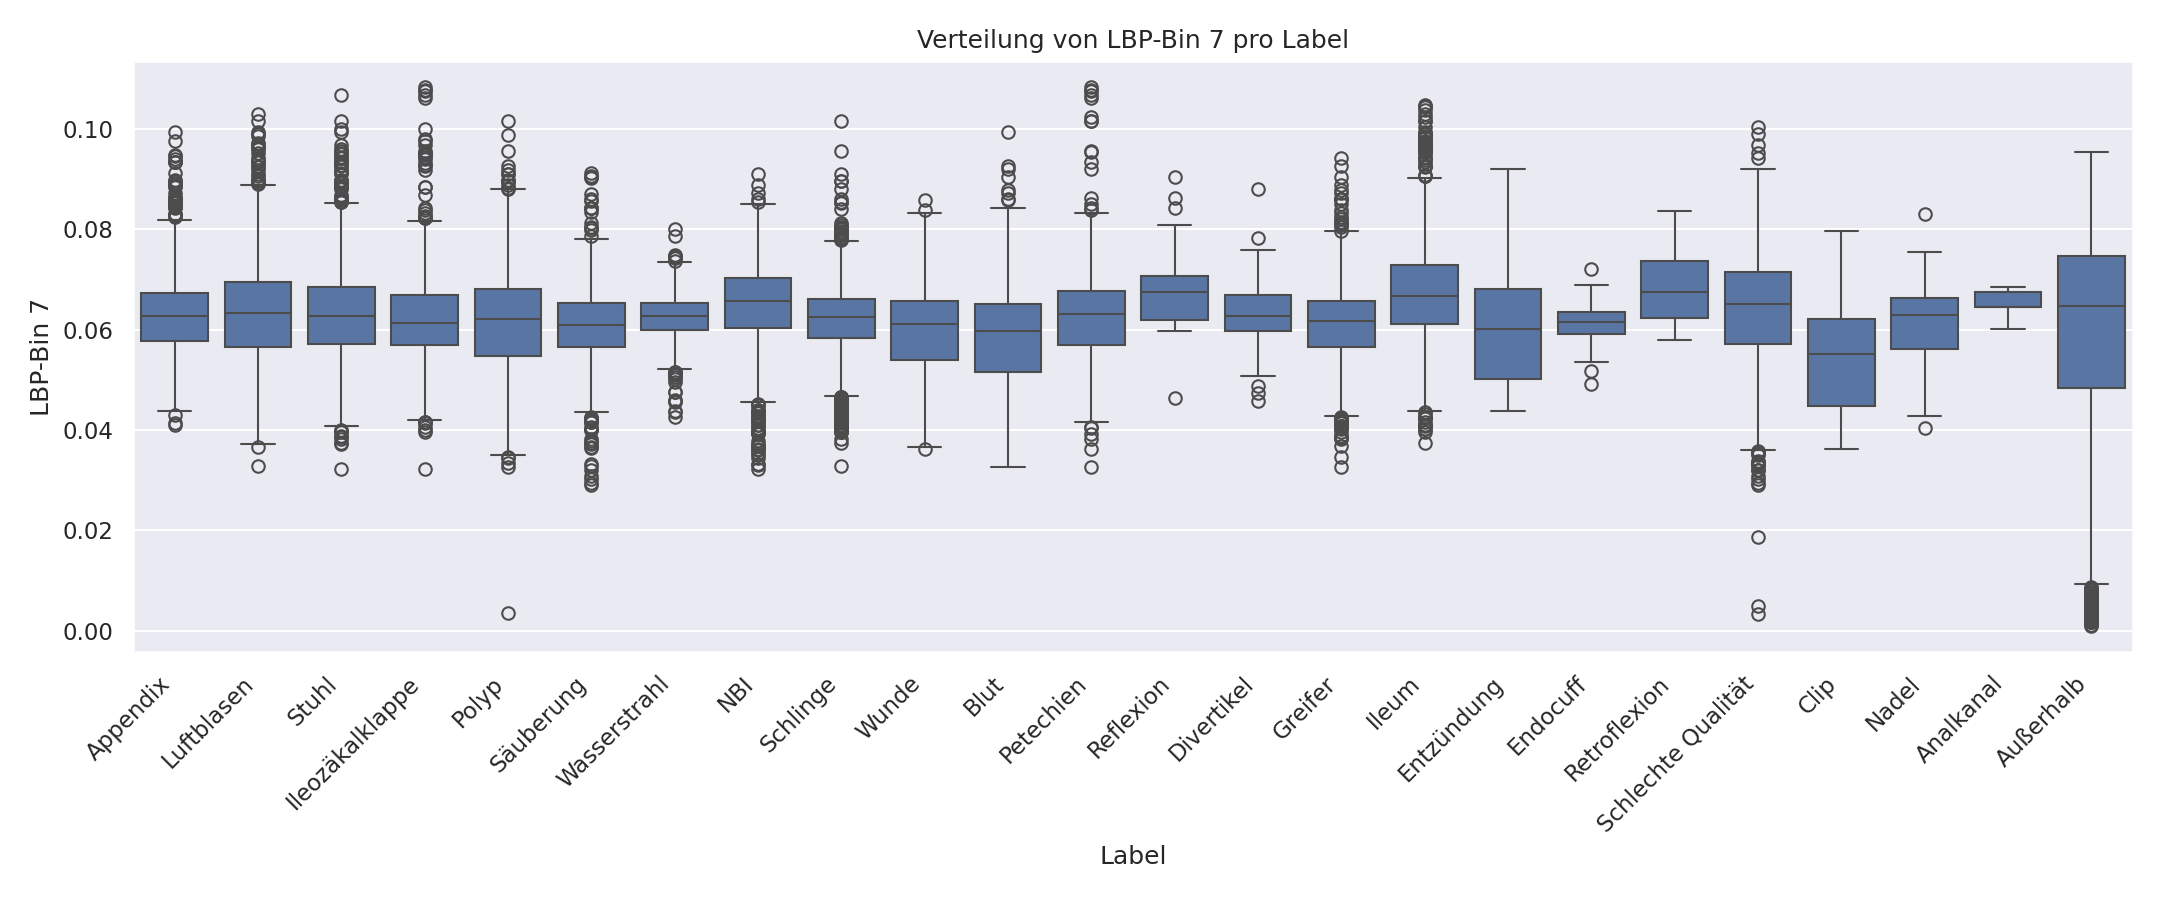
\includegraphics[width=0.9\textwidth]{Images/boxplot_texture_lbp_bin_7.png}
    \caption{Boxplot des LBP-Bins 7.}
\end{figure}

\begin{figure}[p]
    \centering
    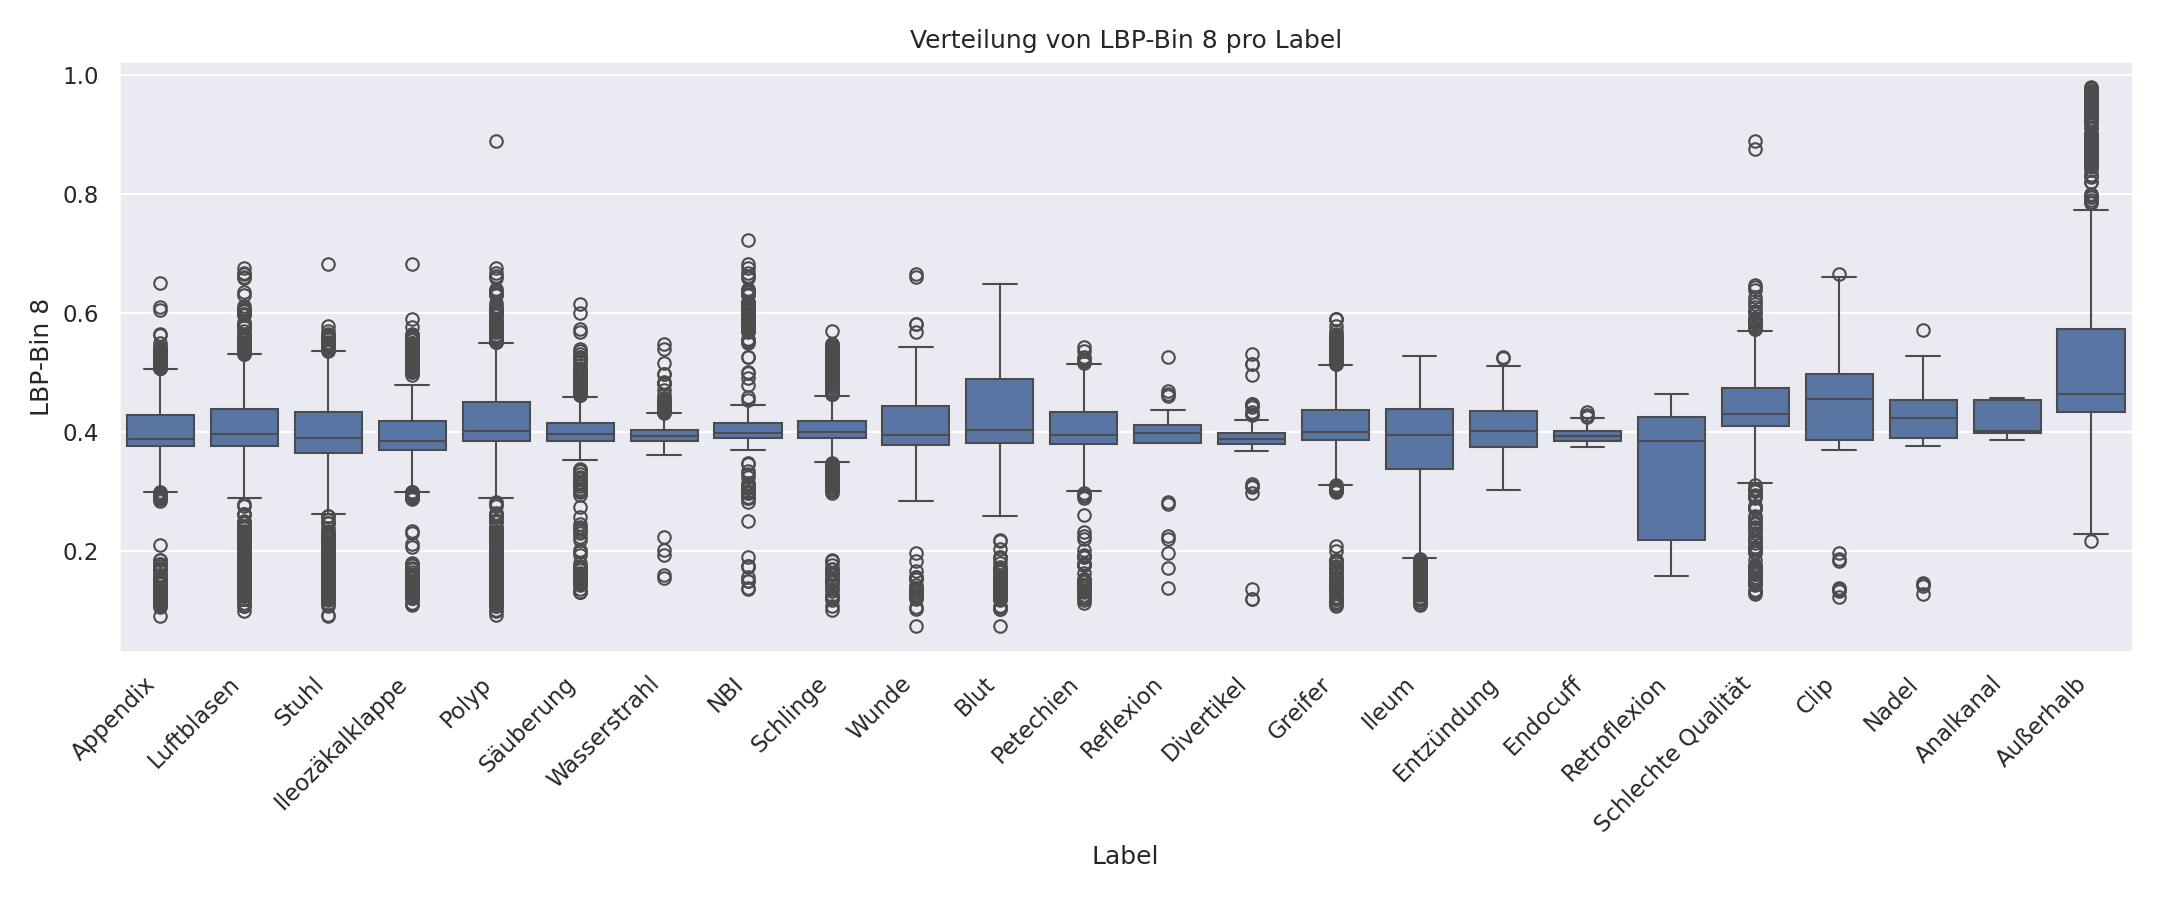
\includegraphics[width=0.9\textwidth]{Images/boxplot_texture_lbp_bin_8.png}
    \caption{Boxplot des LBP-Bins 8.}
\end{figure}

\begin{figure}[p]
    \centering
    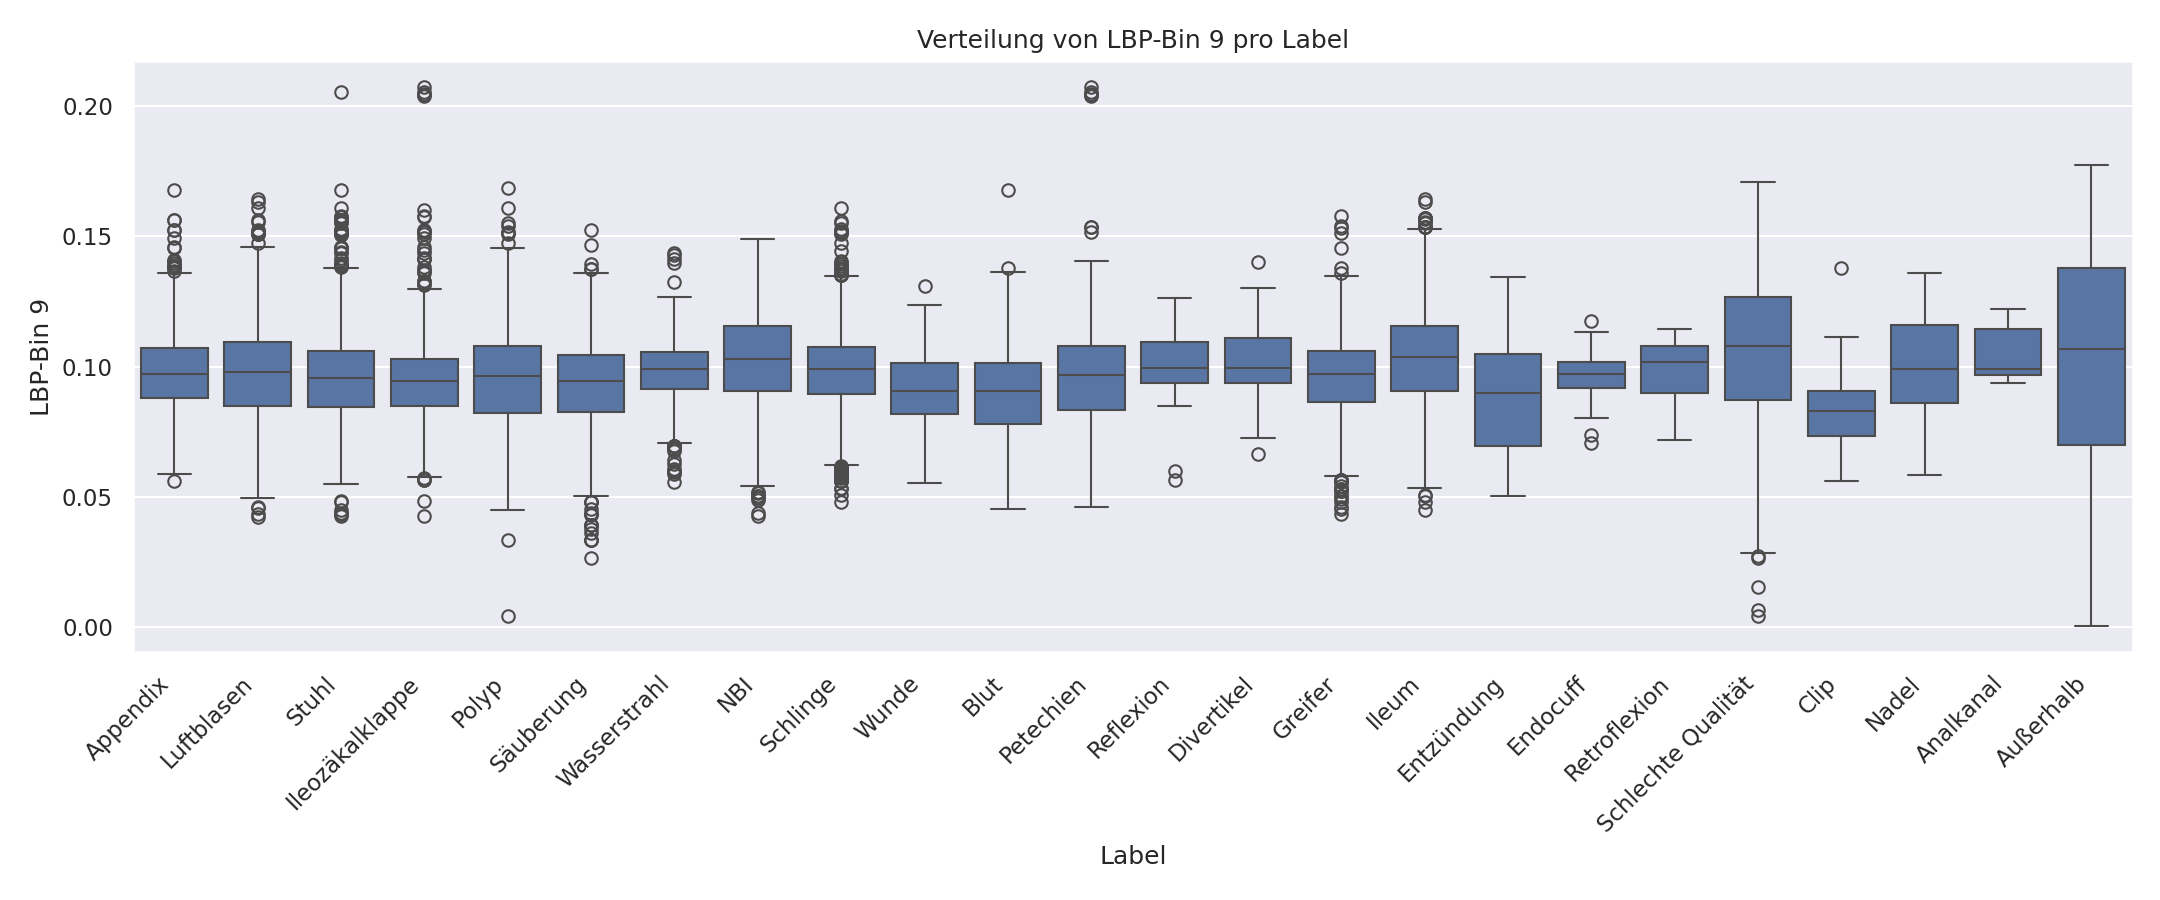
\includegraphics[width=0.9\textwidth]{Images/boxplot_texture_lbp_bin_9.png}
    \caption{Boxplot des LBP-Bins 9.}
\end{figure}
